\documentclass[../../main.tex]{subfiles}
% \documentclass[a4paper,10pt]{ltjsarticle}
\begin{document}
\rhead{京都大学後期$1991$年$5$番}
\setcounter{equation}{0}
\begin{oframed}
  \documentclass[../../main.tex]{subfiles}
\begin{document}

$1$から$n$までの相異なる$n$個の自然数$(n\ge 4)$の中から無作為に$2$個を取り出し，大きい方を$X_1$，小さい方を$Y_1$とする．
つぎに残りの$(n-2)$個の自然数の中から無作為に$2$個を取り出し，大きい方を$X_2$，小さい方を$Y_2$とする．
\begin{enumerate}
  \item $X_1+Y_1$の期待値を求めよ
  \item $X_1$の期待値を求めよ．
  \item $Y_2$の期待値を求めよ．
\end{enumerate}

\end{document}

\end{oframed}
\setlength{\columnseprule}{0.4pt}
\begin{multicols}{2}
  {\bf [解答]}

  \begin{figure}[H]
    \centering
    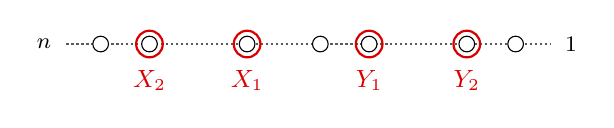
\begin{tikzpicture}[x=0.62cm, y=1cm, every node/.style={font=\small}]
      % 原稿どおり左から X_2, X_1, Y_1, Y_2 の順に並べる（左ほど大きい数）．
      \draw[densely dotted, thick, gray!70!black] (-0.7,0) -- (9.2,0);
      \foreach \x in {0,4.5,8.5} {
        \node[circle, draw, fill=white, inner sep=2pt] at (\x,0) {};
      }
      \foreach \x/\lab in {1/X_2,3/X_1,5.5/Y_1,7.5/Y_2} {
        \node[circle, draw, fill=white, inner sep=2pt] at (\x,0) {};
        \node[circle, draw, thick, red!85!black, inner sep=3.4pt] at (\x,0) {};
        \node[below=6pt, red!85!black] at (\x,0) {$\lab$};
      }
      \node[left=2pt, font=\footnotesize] at (-0.7,0) {$n$};
      \node[right=2pt, font=\footnotesize] at (9.2,0) {$1$};
    \end{tikzpicture}
    \caption{取り出す$4$個の数の様子}
    \label{1991-5:fig:1}
  \end{figure}

  \paragraph{(1)}
  $E(X_1+Y_1)$ は $n$個の自然数から二つを取り出す${}_n C_2$ 通り全てについての和である．
  この時各数字は $n-1$ 回出るので
  \begin{align}
    E(X_1+Y_1)
    & = \dfrac{1}{{}_n C_2} \sum_{k=1}^n k(n-1) \\
    & = n+1
  \end{align}
  が求める期待値である．  $\cdots$(答)

  \vspace{10pt}
  \paragraph{(2)}
  $X_1=k\, (k=2,3,\cdots, n)$となる場合の数は，$k-1$以下の自然数から$Y_1$を選ぶ${}_{k-1}C_{1}$通りである．
  全体の場合の数は(1)より${}_n C_2$通りだから，$E(X_1)$は
  \begin{align}
    E(X_1) & = \sum_{k=2}^{n} \dfrac{k \cdot {}_{k-1} C_1}{{}_n C_2}                                                      \\
    & = \dfrac{1}{{}_n C_2} \sum_{k=2}^n 2 \cdot {}_k C_2 \quad (\because {}_n C_r = \dfrac{n}{r} {}_{n-1} C_{r-1}) \\
    & = \dfrac{4}{n(n-1)} {}_{n+1} C_3 \quad (\because \sum_{k=r}^{n} {}_k C_r = {}_{n+1} C_{r+1})                \\
    & = \dfrac{4}{n(n-1)} \dfrac{(n+1)n(n-1)}{3 \cdot 2 \cdot 1}                                                    \\
    & = \dfrac{2(n+1)}{3}
  \end{align}
  と求まる．$\cdots$(答)

  \vspace{10pt}
  \paragraph{(3)}
  先に $(X_1, Y_1)$ をえらんでも $(X_2, Y_2)$ えらんでも良いので，これらは対称である．
  従って，$Y_2$の期待値と$Y_1$の期待値は等しい．
  そこで$Y_1$について考える．
  期待値の和の公式より
  \begin{align}
    E(X_1+Y_1) = E(X_1) + E(Y_1)
  \end{align}
  であるから，(1)と(2)の結果を代入して
  \begin{align}
    E(Y_2)
    & = E(Y_1) \\
    & = E(X_1+Y_1)- E(X_1) \\
    & = \dfrac{1}{3}(n+1)
  \end{align}
  である．$\cdots$(答)

  \vspace{10pt}
  {\bf [解説]}
  (2)を先に出してもよい．その場合$E(Y_1)$は以下のように求まる．
  $Y_1=k$ なる確率と，$X_1=n+1-k$ なる確率は明らかに等しいから，
  \begin{align}
    E(Y_1)
    & = n+1 - E(X_1)     \\
    & = \dfrac{1}{3}(n+1)
  \end{align}
  である．

  類題として，$1$から$n$の$n$個の自然数から，$m$個をえらぶことを考える．
  小さい方から $k$番目の期待値は
  \begin{align}
    E_k & = \dfrac{k(n+1)}{m+1}
  \end{align}
  で与えられる．

  \begin{figure}[H]
    \centering
    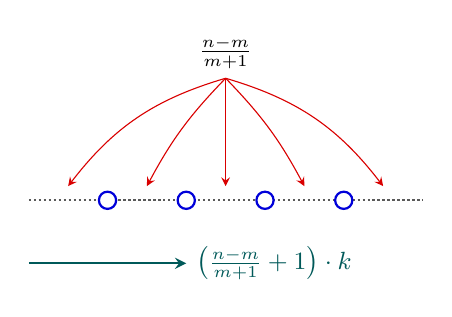
\begin{tikzpicture}[x=1cm, y=1cm, >=stealth, every node/.style={font=\small}]
      % 選んだ m 個（図では 4 個）が残りの n-m 個を m+1 個の隙間に分け，
      % 各隙間には平均 (n-m)/(m+1) 個が入る．
      \coordinate (T) at (2.5,1.55);
      \draw[densely dotted, thick, gray!70!black] (0,0) -- (5,0);
      \foreach \x in {1,2,3,4} {
        \node[circle, draw, thick, blue!85!black, fill=white, inner sep=2.2pt] at (\x,0) {};
      }
      \node[above] at (T) {$\frac{n-m}{m+1}$};
      \foreach \x/\b in {0.5/18,1.5/8,2.5/0,3.5/-8,4.5/-18} {
        \draw[->, red!85!black] (T) to[bend right=\b] (\x,0.18);
      }
      \draw[->, thick, teal!70!black] (0,-0.8) -- (2,-0.8);
      \node[right, teal!70!black] at (2,-0.8)
      {$\left(\frac{n-m}{m+1}+1\right)\cdot k$};
    \end{tikzpicture}
    \caption{一般化における要素の配置の模式図}
    \label{1991-5:fig:2}
  \end{figure}

  $k=1, m$についての証明は容易である．$k=m$の方は，本解説と同様に
  \begin{align}
    E_{m}
    & = \sum_{k=m}^n \dfrac{k \cdot {}_{k-1}C_{m-1}}{{}_n C_m} \\
    & = \dfrac{1}{{}_n C_m} \sum_{k=m}^n m \cdot {}_{k}C_{m} \quad (\because {}_n C_r = \dfrac{n}{r} {}_{n-1} C_{r-1}) \\
    & = \dfrac{m}{{}_n C_m} {}_{n+1}C_{m+1} \quad (\because \sum_{k=r}^n {}_k C_r =  {}_{n+1} C_{r+1})       \\
    & = \dfrac{m}{{}_n C_m} \dfrac{(n+1)!}{(m+1)!(n-m)!} \\
    & = \dfrac{m(n+1)}{m+1}
  \end{align}
  となる．
  対称性から $E_{1} = n+1-E_{m}$ となることに注意して
  \begin{align}
    E_{1} = \dfrac{n+1}{m+1}
  \end{align}
  となる．以上から$k=1,m$では示された．

  % TODO :: 一般の証明を与える

  % TODO :: Cの公式

  \begin{itemize}
    \item ${}_n C_r = {}_{n} C_{n-r}$
    \item $\sum_{k=r}^n {}_k C_r = {}_{n+1} C_{r+1}$
  \end{itemize}

  \newpage
\end{multicols}
\end{document}
